\section{NAX核心设计}
\subsection{目标和原则}
\subsubsection{设计目标}
在设计Token Economy时,为了达到激活生态的目的,每一项规则,无论是增发,销毁,使用场景等需要符合一些基本原则和目标:

\begin{enumerate}[a.]
    \item 公平受益
    \item 正向激励,激励需要持续,规模适当
    \item 治理的有效凭证
    \item 具体持有价值
\end{enumerate}

\subsubsection{设计原则}
为了达到上述的设计目标,我们先从宏观经济模型中寻找一些可用的通用型经济规律。描述一个宏观经济体,为了促进经济体的繁荣发展,需要找到一些有意思的方向。从费雪公式中:

\begin{equation}
M * V = P * T
\end{equation}

\(M\)是Token数量,\(V\)是Token流通速度,\(P\)是Token价格,而\(T\)是系统内总交易额。

很好理解,等式两边其实算的都是以Token数量为计量的GDP。左边\(M * V\)是个数乘以流通速度等于GDP(Token计量),右边总GDP(法币计量)除以Token价格(法币计量)也等于GDP(Token计量)。

我们不难得出,增加Token的“持币价值”是最终有效促进经济体有效途径,然后增加Token的持有价值有如下方法:

\begin{enumerate}[a.]
	\item 系统设计逻辑简洁有效
	\item 增加质押、减少过多的流通量
	\item 提高非交易地址优势
	\item 增加持有NAS和NAX地址数
	\item 增加Token使用场景
\end{enumerate}

\subsection{NAX核心逻辑}

\subsubsection{资产公平和有效性}

一个公平有效的Token Economy应该是一个权益的产生是一个规则清晰,信息对称通证系统。因此,NAX的增发方式将只采用通过质押NAS(Staking)的方式获得。通过Staking的单一的增发形式,可以保证资产的相对公平性,不容易因为合约或是规则的漏洞使得系统出现严重错配的现象。NAS的持有者通过锁住token的流通性以获取NAX的权益。这样使得在现有NAS的经济体系里,是相对公平和公正的。

\subsubsection{星云式质押 -- Smart Staking}
传统的质押方式是用户将资产转入到智能合约当中暂为保管,并记录质押相关的系统。但是这样中心化质押方式,使得大量的资产安全问题维系在一个智能合约里,2016年以太坊的The DAO攻击就是利用了对合约漏洞的攻击,使得The DAO里面的资产被盗走。星云链一直坚持区块链的核心的理念和精神:用户的资产神圣不可侵犯。

Staking的核心目的是锁住资产的流通性,并不是资产本身,更不应该转移资产的所属权。因此,我们提出一种不转移资产的质押方式,我们称之为星云式质押 -- Smart Staking。用户只需要与质押合约签订一个契约,系统就认为用户参与的质押,但并不需要用户转移资产进入合约。然后合约会每天不定时间的检查用户帐户里的资产是否与契约相符合,如果资产少于契约的数量,将会视为自动放弃质押,同时也不俱备进一步获得增发收益的权益。

\subsubsection{NAX增发规则}
NAX的核心系统将以每6,000高度(一天左右)作为一个增发周期。每个周期将根据有一个固定的待增发量,当去的质押比率情况进行不同程度的增发。每周期过后,增发参数将以一程度衰减。一个直观的效果,经过一年之后,增发系数将会衰减到初始的一半左右。

公式如下:

\begin{equation}
  K_{i,j} = \frac{P_{i,j} T_{i,j}}{\sum_j P_{i,j} T_{i,j}} \lambda_i C_i
\end{equation}

其中,
\begin{enumerate}
   \item \(K_{i,j}\): 第\(i\)期用户\(j\)获得的Token数量
   \item \(P_{i,j}\): 第\(i\)期用户\(j\)的质押量
   \item \(T_{i,j}\): 第\(i\)期用户\(j\)的质押时间
   \item \(C_i\): 第\(i\)期初始总增发量,\(C_i=C_0 \mu^i\),增发衰减系数$\mu=0.9981$
   \item \(\lambda_i\): 第\(i\)期增发比例,\(\lambda_i = f(x_i)\),总质押量\(x_i = \sum_j P_{i,j} T_{i,j}\),其中
     \begin{equation}
       f(x) = \frac{x^2}{x_c^2+x^2}
     \end{equation}
     其中\(x_c\)是一个常数,为总质押量比较典型的取值,增发比例与总质押量的关系如图\ref{func}所示。可见增发比例的取值在0到1之间,随总质押量的增大而增大并不断趋于1,在\(x_c\)之前增发比例随总质押量的增大而较快地增大,而在\(x_c\)之后增发比例随总质押量的增大而缓慢增大。
    \begin{figure}
      \centering
      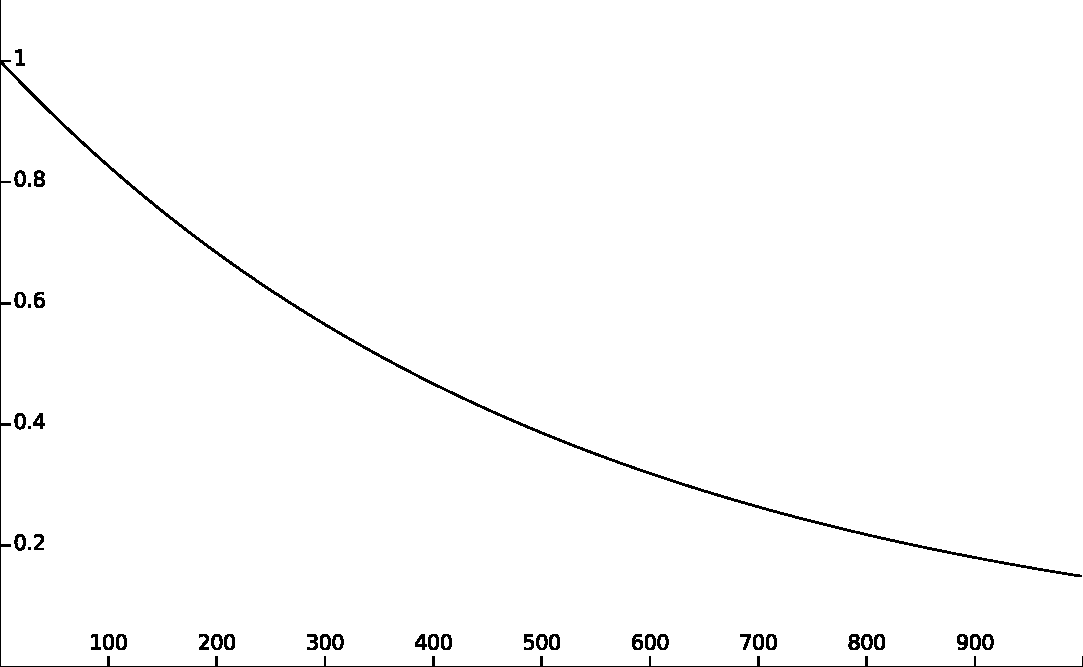
\includegraphics[scale=0.4]{../common/ch/everyday.pdf}
      \caption{每日增发衰减示意图}\label{func}
    \end{figure}
    \begin{figure}
      \centering
      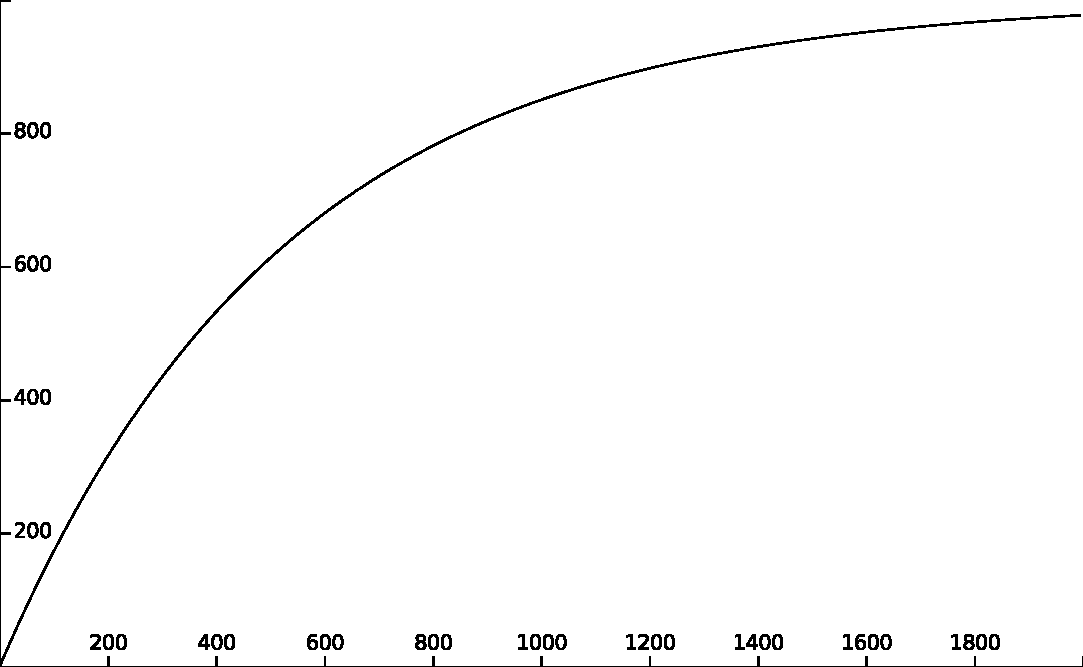
\includegraphics[scale=0.4]{../common/ch/acc.pdf}
      \caption{累积增发NAX数量}\label{acc}
    \end{figure}
  %\item 质押池相比总流通量的比率:$\alpha$
\end{enumerate}
由于\(\lambda_i \le 1\),每一期的增发量有上界
\begin{equation}
  \sum_j K_{i,j} = \frac{\sum_j P_{i,j} T_{i,j}}{\sum_j P_{i,j} T_{i,j}} \lambda_i C_i = \lambda_i C_i \le C_i
\end{equation}
所以总发行量有上界
\begin{equation}
  \sum_{i,j} K_{i,j} \le \sum_i C_i = \sum_i C_0 \mu^i = \frac{C_0}{1-\mu}
\end{equation}
令此上界为100亿(\(10^{10}\)),可解出\(C_0 = 10^{10}(1-\mu) = 1.9\times10^7\)。


同一个周期内,系统会根据质押数量以及相应的质押时间长短来分配增发的总量,以达到公平的效果,即质押数量越多,质押时间越长,所分配到的增发数量也会更多。该设计会达到以下博弈场景:
\begin{enumerate}
  \item 早期参与质押的用户,有更大的概率获得更多的系统增发
  \item 随着质押率增加,系统增发数量也会相应提高,以鼓励更多人加入质押
\end{enumerate}

\subsection{合约框架}
NAX是由一组合约组成,是在NRC20基础上扩展的合约组,并配有多签合约管理整个合约里的参数,详细如图\ref{fig:nax_framework}所示。

\begin{figure}[htbp]
  \centering
    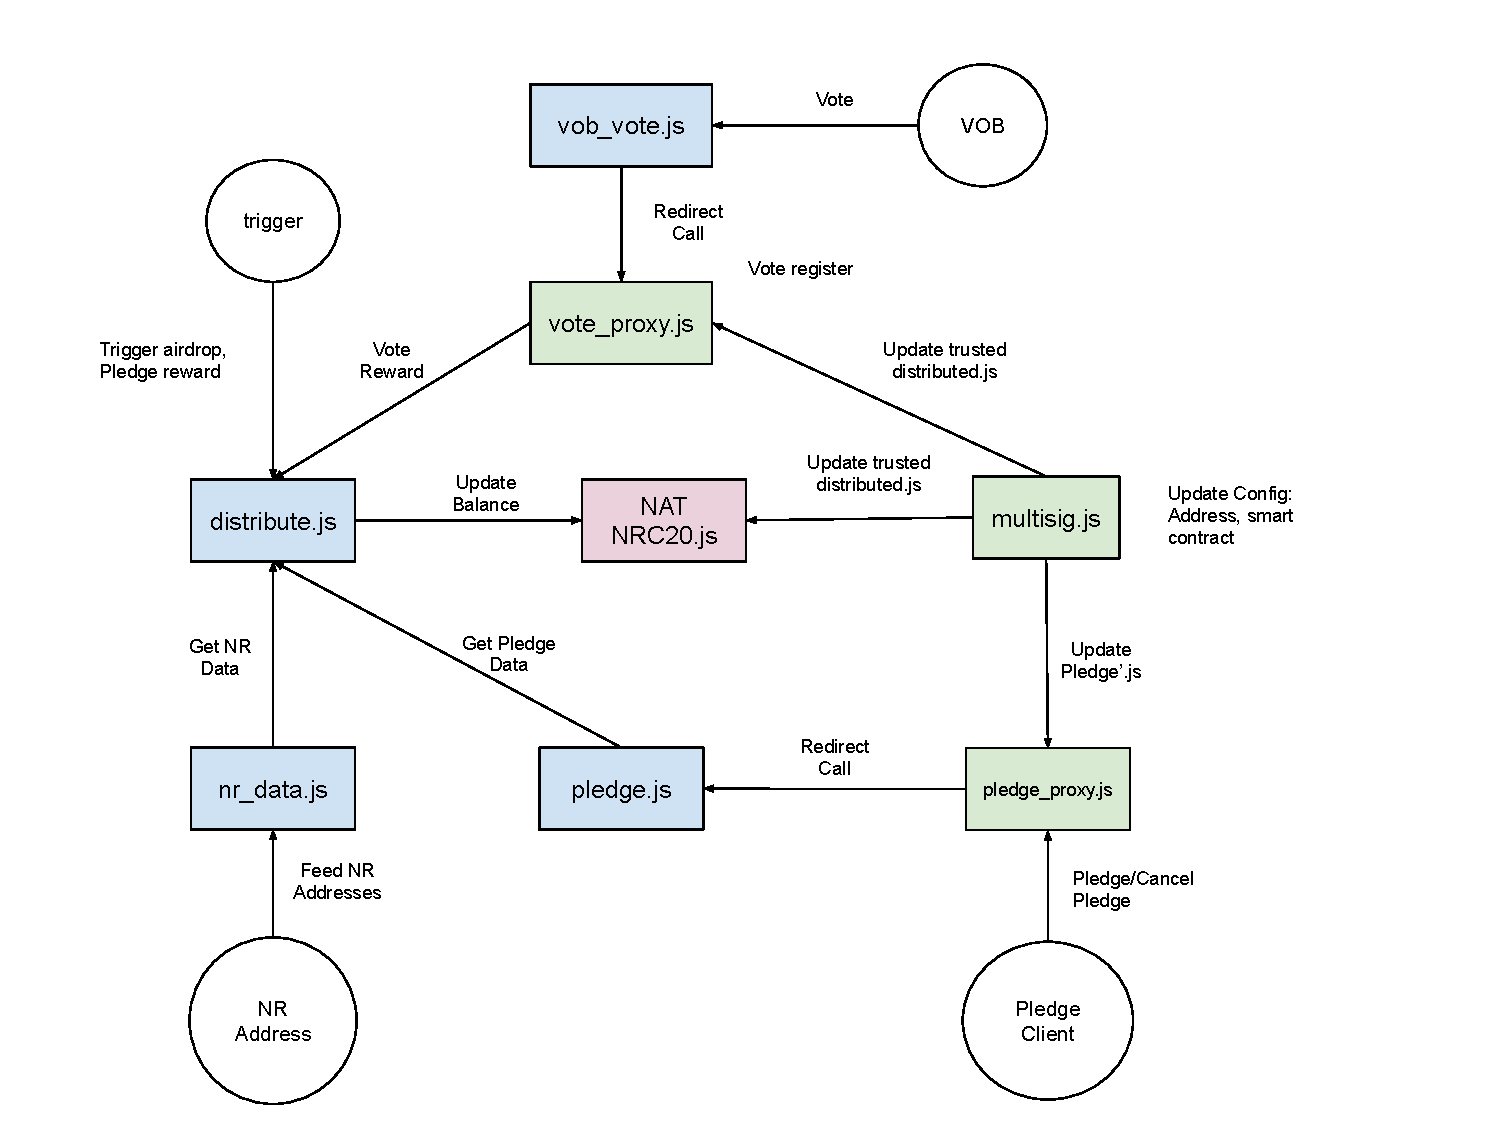
\includegraphics[width=1\textwidth]{../common/ch/nax.pdf}
    \caption{NAX 合约示意图(此图待更新) \label{fig:nax_framework}}
\end{figure}
